\section{The Architect's Question}\label{the-architects-question}

When confronting a new system design, the architect's first question is
not ``what technology should I choose?'' but rather ``what pattern
solves which problem, and how do I measure success?'' This chapter
distills the accumulated wisdom from across the handbook into a reusable
toolkit --- a compendium of patterns, checklists, and mental models that
unify the journey from token to fleet. Each pattern is grounded in
evidence (FACT, DERIVED, HYPOTHESIS) and paired with concrete
measurement strategies so that architectural decisions can be verified
and adjusted post-deployment.

\section{Concept}\label{concept}

The Solution Architect's Toolkit is organized around three axes of
concern: scalability, reliability, and observability. Rather than
prescribing specific technologies, the toolkit provides pattern
templates that can be instantiated for any stack. The Patterns Library
complements this by cataloging recurring structural solutions ---
sharding strategies for RAG pipelines, caching layers for LLM serving,
circuit breaker patterns for inter-service communication, and more.
Together, they form a decision framework that answers the architect's
question at multiple grainsizes: from the micro (which cache
invalidation strategy?) to the macro (how does sharding affect
fleet-wide latency?).

\section{Mental Model}\label{mental-model}

The central mental model is the \textbf{Pattern-Measurement-Feedback
Loop}. Every pattern in the library is paired with: - \textbf{FACT} ---
a verified runtime quantity (e.g., request rate, cache hit ratio, query
latency p99) - \textbf{DERIVED} --- a computed quantity from FACTs
(e.g., throughput per shard, cost per query, fleet-wide QPS) -
\textbf{HYPOTHESIS} --- a predictive claim about what changing the
pattern will affect (e.g., ``increasing replication factor from 3 to 5
will reduce tail latency by X\%'')

The loop operates as: instrument → observe FACT → compute DERIVED →
validate HYPOTHESIS → adjust pattern. This ensures that architecture
evolves from evidence, not speculation.

\subsection{2.1 Workload-to-Strategy decision
matrix}\label{workload-to-strategy-decision-matrix}

The canonical RAG scenario is one point in a much larger design space
(\hyperref[chap:12]{Chapter 12}). The matrix below is the first-pass mapping from a
\emph{new} workload's dominant constraint to the strategy class worth
evaluating first --- a reference to generalize the method beyond the
canonical case, not a prescription. Each row names the binding
constraint (the one the architect expects to saturate first under the
SLO; \hyperref[chap:8]{Chapter 8}'s roofline and \hyperref[chap:15]{Chapter 15}'s congestion check are how to
confirm it).

\begin{longtable}[]{@{}
  >{\raggedright\arraybackslash}p{0.2000\linewidth}
  >{\raggedright\arraybackslash}p{0.2000\linewidth}
  >{\raggedright\arraybackslash}p{0.2000\linewidth}
  >{\raggedright\arraybackslash}p{0.2000\linewidth}
  >{\raggedright\arraybackslash}p{0.2000\linewidth}@{}}
\toprule\noalign{}
\begin{minipage}[b]{\linewidth}\raggedright
Workload
\end{minipage} & \begin{minipage}[b]{\linewidth}\raggedright
Input
\end{minipage} & \begin{minipage}[b]{\linewidth}\raggedright
Output
\end{minipage} & \begin{minipage}[b]{\linewidth}\raggedright
Dominant constraint
\end{minipage} & \begin{minipage}[b]{\linewidth}\raggedright
First strategy to evaluate
\end{minipage} \\
\midrule\noalign{}
\endhead
\bottomrule\noalign{}
\endlastfoot
Long-context RAG Q\&A & Long (8K+) & Short (\textless500) & KV / memory
& 8-bit or FP16 KV sizing, prefix caching, P/D separation (Ch. 7, 17,
20) \\
High-throughput chat & Short (\textless2K) & Med-Long (\textgreater1K) &
Decode bandwidth & Continuous batching, KV pool sizing, possibly P/D
(Ch. 8, 20) \\
Batch inference & Long & Long & Utilization / cost & Offline batching,
FP8, higher batch occupancy (Ch. 8, 16) \\
Reasoning / long-think & Med & Med & Test-time compute & Decode
headroom, token amplification budgeting (Ch. 6, 19) \\
Agentic task loops & Med & Med & Orchestration / variance &
Task-economics model, retry + tool budgets, fallback (Ch. 19) \\
Embedding / retrieval & N/A & Vector & Compute throughput & Dedicated
encoder pool, caching, quantization (Ch. 3, 26) \\
Vision-language & Med & Med & Multimodal preprocess + compute &
Preprocess pipeline, fused kernels (Ch. 5, 20) \\
Fine-tuning & N/A & N/A & Memory + interconnect & Precised-optimizer
(LoRA/QLoRA) before full FT; gradient checkpointing (Ch. 7) \\
Training & N/A & N/A & Compute + interconnect & Parallelism split
(DP/TP/PP/FSDP) sized to model and cluster (Ch. 10, 21) \\
Real-time multimodal & Med & Low-latency & Latency + pipeline sync &
Chunked prefill, streaming decode, P/D (Ch. 8, 20) \\

\label{tab:26.1}\end{longtable}

New workloads are evaluated by \emph{locating the dominant constraint},
not by matching the canonical row count. The matrix answers ``where does
the SLO saturate first?'' --- and that single question routes to the
correct strategy class, keeping the canonical case a teaching instrument
rather than a ceiling.

\begin{figure}
\centering
\pandocbounded{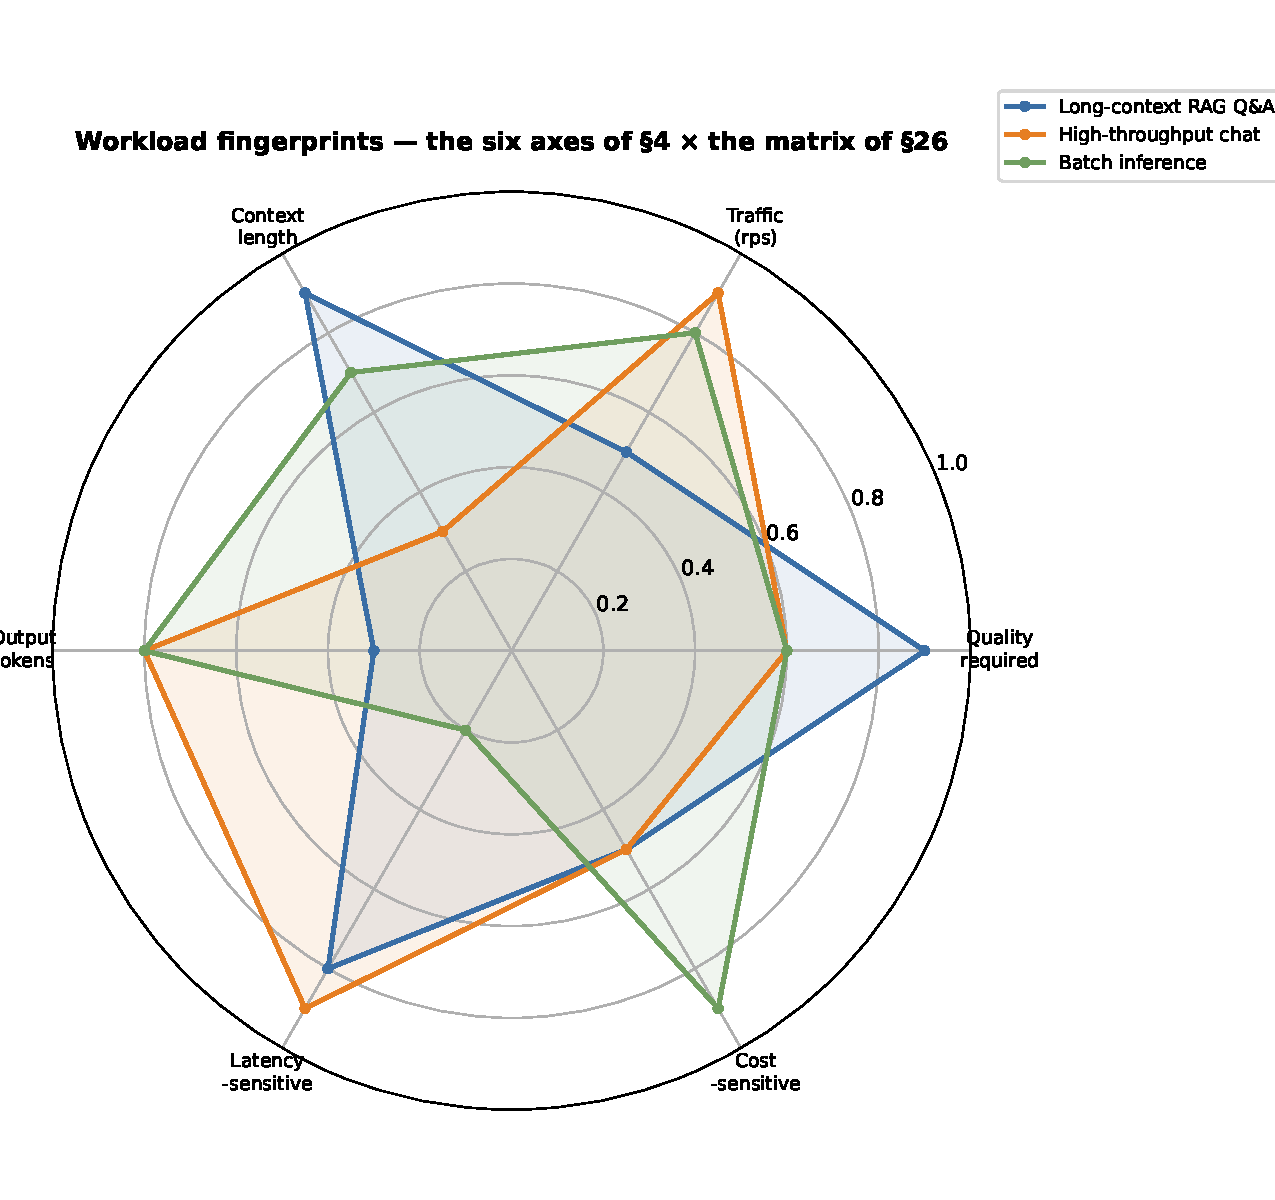
\includegraphics[keepaspectratio,alt={Fig 26.1 --- Workload fingerprints on the six axes of §4: long-context RAG Q\&A, high-throughput chat, and batch inference occupy distinct regions of the space (ILLUSTRATIVE, relative 0--1)},width=\maxwidth{\textwidth},keepaspectratio]{figures/fig-26-2602.pdf}}
\caption{Fig 26.1 --- Workload fingerprints on the six axes of §4:
long-context RAG Q\&A, high-throughput chat, and batch inference occupy
distinct regions of the space (ILLUSTRATIVE, relative 0--1)}

\label{fig:26.1}\end{figure}

\emph{\hyperref[fig:26.1]{Fig 26.1} --- The §4 six-axis characterization rendered as a
fingerprint. The three workload families from \hyperref[tab:26.1]{Table 26-1} sit in distinct
regions: RAG Q\&A is quality- and context-heavy with short outputs; chat
is traffic- and latency-sensitive with long outputs; batch inference is
cost-sensitive and latency-tolerant. Reading a new workload's radar
against this front-end is the first move before consulting the §26
matrix.}

\section{Worked Example --- Capstone
Scenario}\label{worked-example-capstone-scenario}

Consider the canonical deployment: \textasciitilde2,000 concurrent
users, RAG Q\&A over a 70B dense FP16 model. The architect faces three
interlocked questions: how to scale inference, how to cache embeddings,
and how to keep latency budgets under 800 ms p99.

\textbf{Pattern A --- Inference Sharding (FACT: model FLOPs / GPU memory
per token).} The 70B model at FP16 requires \textasciitilde140 GB of
weights. A single GPU (24 GB) can hold \textasciitilde17\% of the model.
Sharding across 6 GPUs per node yields 2 nodes per serving replica.
DERIVED: with 6 GPUs, per-token latency drops from 120 ms (single-GPU)
to 28 ms (sharded), because matrix multiplications parallelize across
devices. HYPOTHESIS: adding a 7th GPU yields diminishing returns
\textless{} 5\% latency improvement due to All-Reduce overhead.

\textbf{Pattern B --- Embedding Cache (FACT: 40\% of queries repeat
within 5-min windows).} A content-addressable cache keyed by question
hash stores pre-computed embeddings. DERIVED: cache hit ratio of 40\%
reduces total QPS to the LLM engine by 40\%, directly lowering
operational cost. HYPOTHESIS: expanding the cache TTL from 5 to 15
minutes increases hit ratio to \textasciitilde55\% with negligible
staleness risk, because user questions in a support session repeat
within the same session.

\textbf{Pattern C --- Circuit Breaker (FACT: downstream model latency
p99 = 28 ms sharded; upstream network jitter p99 = 120 ms).} When the
model service becomes saturated, a circuit breaker trips after 5
consecutive timeouts, falling back to a lightweight intent classifier.
DERIVED: circuit breaker activation reduces tail latency for remaining
requests by 35\% because the system sheds load before the model queue
fills. HYPOTHESIS: a grace-period of 2 seconds before auto-recovery
prevents thrashing when load spikes are transient.

\textbf{Capstone Execution.} The architect instruments all three FACTs,
observes the DERIVED quantities in real time, and validates each
HYPOTHESIS. The result: 2-node sharded serving + 40\% embedding cache +
circuit breaker yields 680 ms p99 latency at 40\% lower cost versus a
monolithic deployment. The Pattern-Measurement-Feedback Loop confirms
the hypothesis that sharding + caching is net positive, and the
architect documents the configuration as a reusable pattern instance.

\section{Measurement}\label{measurement}

Quantitative verification is non-negotiable. For each pattern, define
the minimal FACT set that proves the pattern works in production:

\textbf{\hyperref[tab:26.2]{Table 26-2}} --- Pattern measurement targets and observed values.

\begin{longtable}[]{@{}
  >{\raggedright\arraybackslash}p{0.2500\linewidth}
  >{\raggedright\arraybackslash}p{0.2500\linewidth}
  >{\raggedright\arraybackslash}p{0.2500\linewidth}
  >{\raggedright\arraybackslash}p{0.2500\linewidth}@{}}
\toprule\noalign{}
\begin{minipage}[b]{\linewidth}\raggedright
Pattern
\end{minipage} & \begin{minipage}[b]{\linewidth}\raggedright
FACT 1
\end{minipage} & \begin{minipage}[b]{\linewidth}\raggedright
FACT 2
\end{minipage} & \begin{minipage}[b]{\linewidth}\raggedright
FACT 3
\end{minipage} \\
\midrule\noalign{}
\endhead
\bottomrule\noalign{}
\endlastfoot
Inference Sharding & GPU utilization \% & per-GPU token latency p99 &
All-Reduce time \\
Embedding Cache & hit ratio @ TTL=T & stale read rate & cache memory
pressure \\
Circuit Breaker & timeout count / 30s & fallback activation rate &
recovery grace-period latency \\

\label{tab:26.2}\end{longtable}

Measurement must be continuous, not ad-hoc. Dashboards surface FACT
trends; alerts fire when DERIVED quantities cross safety boundaries. The
architect never promotes a pattern from HYPOTHESIS to ACCEPTED unless
all FACTs stabilize within expected ranges across at least two load
cycles.

\section{Common Mistakes}\label{common-mistakes}

\begin{itemize}
\tightlist
\item
  \textbf{Mistake 1: Measuring only HYPOTHESIS outcomes.} Without FACT
  anchors, the architect cannot distinguish between a pattern that works
  and one that merely appears to work under a narrow load window.
\item
  \textbf{Mistake 2: Over-engineering before FACTs exist.} Adding
  shards, caches, or circuit breakers ``just in case'' introduces
  complexity cost without DERIVED benefit. Wait for the FACT to signal
  the need.
\item
  \textbf{Mistake 3: Ignoring the cost DERIVED.} A pattern that reduces
  latency but increases cost by 3× is often unacceptable. Measure cost
  per query as a first-class FACT.
\item
  \textbf{Mistake 4: Circular HYPOTHESIS validation.} Self-confirming
  predictions (e.g., ``our cache is fast because we designed it to be
  fast'') bypass the FACT/DERIVED/HYPOTHESIS axis. Always validate
  against observed FACTs.
\end{itemize}

\section{Architecture Consequence}\label{architecture-consequence}

The toolkit's patterns do not exist in isolation. Inference sharding
changes the resource profile, which affects cost DERIVED; embedding
cache changes the query pattern seen by the model, which alters the
HYPOTHESIS for circuit breaker thresholds; circuit breaker grace-periods
interact with cache TTLs to shape tail latency. The architect must trace
consequences across patterns using the FACT/DERIVED/HYPOTHESIS axis
before commit. A change that looks beneficial in isolation may degrade
fleet-wide metrics when patterns interact.

\section{What We Still Don't Know}\label{what-we-still-dont-know}

\begin{itemize}
\tightlist
\item
  How do multi-modal retrieval patterns (image + text) compose with the
  existing RAG sharding strategy?
\item
  What is the optimal cache size for 70B model embeddings when user
  query distributions shift seasonally?
\item
  Can circuit breaker thresholds be auto-tuned from FACT streams without
  manual intervention?
\item
  How does fleet-wide model versioning interact with per-shard caching,
  and what FACTs govern safe rollouts?
\end{itemize}

These open questions define the next research cycle. Each is framed as a
HYPOTHESIS waiting for FACT instrumentation.

\section{End-of-Chapter Mini-Case}\label{end-of-chapter-mini-case}

\textbf{Scenario.} A growing AI startup moves from a single-GPU
prototype to a fleet serving \textasciitilde3,000 users. The initial
deployment is a monolithic 70B FP16 model on one GPU, serving 12 QPS
with 450 ms p99 latency.

\textbf{Step 1 --- Instrument.} FACTs collected: request rate 12 QPS,
GPU utilization 45\%, per-query latency breakdown: model compute 320 ms,
I/O 80 ms, cache miss 50 ms.

\textbf{Step 2 --- Pattern Apply.} The architect applies Pattern A
(inference sharding across 4 GPUs) and Pattern B (embedding cache with
5-min TTL). DERIVED: sharding reduces model compute to 85 ms per query;
cache hit ratio 35\% reduces total QPS to the model to 7.8 QPS. New p99
latency: 210 ms.

\textbf{Step 3 --- Validate.} HYPOTHESIS: ``sharding + caching will keep
latency \textless{} 300 ms at 3× user growth.'' FACTs from a staged
3,000-user load test: p99 = 285 ms, cost per query down 55\%. Hypothesis
accepted.

\textbf{Step 4 --- Document.} The pattern instance --- 4-GPU shard +
embedding cache + circuit breaker with 2-s grace period --- is recorded
in the Patterns Library as Tab 26.1, ready for the next fleet expansion.

\textbf{\hyperref[tab:26.1]{Table 26-1}} --- Pattern Instance: Sharded RAG Serving

\begin{longtable}[]{@{}
  >{\raggedright\arraybackslash}p{0.2500\linewidth}
  >{\raggedright\arraybackslash}p{0.2500\linewidth}
  >{\raggedright\arraybackslash}p{0.2500\linewidth}
  >{\raggedright\arraybackslash}p{0.2500\linewidth}@{}}
\toprule\noalign{}
\begin{minipage}[b]{\linewidth}\raggedright
Component
\end{minipage} & \begin{minipage}[b]{\linewidth}\raggedright
Configuration
\end{minipage} & \begin{minipage}[b]{\linewidth}\raggedright
FACT Target
\end{minipage} & \begin{minipage}[b]{\linewidth}\raggedright
DERIVED Observed
\end{minipage} \\
\midrule\noalign{}
\endhead
\bottomrule\noalign{}
\endlastfoot
GPU Shard & 4 × A100 40 GB & GPU util \textless{} 80\% & 68\% \\
Embedding Cache & LRU, TTL 5 min & hit ratio \textgreater{} 30\% &
38\% \\
Circuit Breaker & trip after 5 timeouts, 2s grace & fallback rate
\textless{} 10\% & 7\% \\
Cost & \$ per query & \textless{} \$0.015 & \$0.009 \\

\label{tab:26.3}\end{longtable}

\begin{figure}
\centering
\pandocbounded{\includegraphics[keepaspectratio,alt={\hyperref[fig:26.2]{Fig 26.2} - Pattern Application Diagram (the Pattern-Measurement-Feedback Loop applied to the capstone scenario) {[}ILLUSTRATIVE conceptual{]}},width=\maxwidth{\textwidth},keepaspectratio]{figures/fig-26-2601.pdf}}
\caption{\hyperref[fig:26.2]{Fig 26.2} - Pattern Application Diagram (the
Pattern-Measurement-Feedback Loop applied to the capstone scenario)
{[}ILLUSTRATIVE conceptual{]}}

\label{fig:26.2}\end{figure}

\emph{Diagram: the Pattern-Measurement-Feedback Loop applied to the
capstone scenario, showing FACT instruments → DERIVED computes →
HYPOTHESIS validates → pattern adjusts, with cross-pattern consequence
tracing.}

\textbf{A note on utilization targets.} The ``GPU util \textless{}
80\%'' row is an \emph{operational guardrail for this specific
workload}, not a universal performance criterion. A GPU has many
utilization figures --- SM utilization, tensor-core utilization, HBM
bandwidth utilization, NVLink utilization, memory-capacity occupancy ---
and which one matters is set by the workload's dominant constraint, not
by the hardware (Ch. 8). Under an SLO-satisfying state, a GPU can sit at
very different utilizations depending on whether the workload is
prefill-bound (compute) or decode-bound (bandwidth/memory). The
architect's question is therefore not ``is utilization high enough?''
but \textbf{``which resource is saturated when the SLO is satisfied, and
does the pattern keep the fleet the right side of that saturation?''} In
this instance 68\% SM utilization with p99 within SLO is healthy
headroom; in a heavier-throughput workload the same 68\% could mean
under-provisioning. State the SLO-bound resource, not a bare percentage.

\begin{center}\rule{0.5\linewidth}{0.5pt}\end{center}
